% !TEX root= ../main.tex
\section{Graph theories}
\label{sec:Graph theories}
We have just shown that in the case of unrestricted theories, there is no guarantee that an inconsistency is binary-derivable, but what about graph theories?
After all, it is the graph theories that motivated the conjecture in the first place.

It turns out that even for graph theories, some provable NAND-clauses require non-binary NAND-clauses in their proof, i.e they are \textit{not} binary-derivable.
This section will prove the following:
\begin{theorem}
  There exists a graph with vertices $a,b$ such that $\ol{ab}$ is not binary-derivable.
  \label{thm:non_binary_derivable}
\end{theorem}
The theorem will be proven simply by presenting a graph containing a provable binary NAND-clause and show that the only way to prove it is through using non-binary NAND-clauses.
We will then make an attempt to extend the graph, making it inconsistent, and then show that its inconsistency proof has to include the non-binary-derivable NAND-clause.
This attempt will however prove to be unsuccessful.

Let us again consider the graph from Figure~\ref{fig:v3_counter_graph}, Section~\ref{sub:V3 and implication 2}:\par
\begin{figure}[!h]
  \centering
  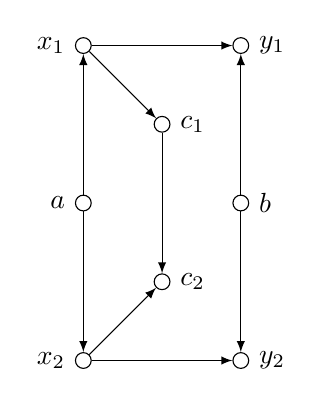
\begin{tikzpicture}
    [
    point/.style={circle,draw,inner sep=0pt,minimum size=2mm}
    ]
    \node (a) at (0,2) [point,label=left:$a$] {};
    \node (x1) at (0,4) [point,label=left:$x_1$] {};
    \node (x2) at (0,0) [point,label=left:$x_2$] {};
    \node (b) at (2,2) [point,label=right:$b$] {};
    \node (y1) at (2,4) [point,label=right:$y_1$] {};
    \node (y2) at (2,0) [point,label=right:$y_2$] {};
    \node (c1) at (1,3) [point,label=right:$c_1$] {};
    \node (c2) at (1,1) [point,label=right:$c_2$] {};
    \draw [-latex] (a) to (x1);
    \draw [-latex] (a) to (x2);
    \draw [-latex] (b) to (y1);
    \draw [-latex] (b) to (y2);
    \draw [-latex] (x1) to (y1);
    \draw [-latex] (x1) to (c1);
    \draw [-latex] (x2) to (y2);
    \draw [-latex] (x2) to (c2);
    \draw [-latex] (c1) to (c2);
  \end{tikzpicture}
  \caption{}
  \label{fig:open_door}
\end{figure}
As before, the vertices $y_1$, $y_2$ and $c_2$ are initial vertices of disjoint rays, and not sinks.

The NAND-clause we will show not to be binary-provable is $\ol{ab}$.
Figure~\ref{fig:v3_counter_proof} proves $\ol{ab}$, but the proof contains two non-binary NAND-clauses.
We will show that this is unavoidable.
In order to do this, we utilize the table from Figure~\ref{fig:v3_counter_table} worked out in Section~\ref{sub:V3 and implication 2}.
We will show it here for convenience.\par
\begin{figure}[!h]
  \centering
  \[\begin{array}{|c||c|c|c|c|c|c|c|c|}
    \hline
    & a & b & x_1 & x_2 & y_1 & y_2 & c_1 & c_2 \\ \hline\hline
    a & \alpha_1 & & & & \alpha_1 & \alpha_1 & \alpha_1 & \alpha_2 \\ \hline
    b &-& \alpha_4 & \alpha_4 & \alpha_3 & & & \alpha_3 & \alpha_4 \\ \hline
    x_1 &-&-& \alpha_4 & & & \alpha_6 & & \alpha_6 \\ \hline
    x_2 &-&-&-& \alpha_5 & \alpha_5 & & \alpha_5 & \\ \hline
    y_1 &-&-&-&-& \alpha_1 & \alpha_1 & \alpha_1 & \alpha_2 \\ \hline
    y_2 &-&-&-&-&-& \alpha_1 & \alpha_1 & \alpha_2 \\ \hline
    c_1 &-&-&-&-&-&-& \alpha_1 & \\ \hline
    c_2 &-&-&-&-&-&-&-& \alpha_4 \\ \hline
  \end{array}\]
  \caption{}
  \label{fig:open_door_table}
\end{figure}

Let us assume that we have a rule application with all binary NAND-clauses in the premise and with $\ol{ab}$ in the conclusion.
Based on the (Rneg)-rule, we know that the premise must contain at least one binary NAND-clause containg $a$ and at least one containing $b$.
The table above tells us that the only provable binary NAND-clauses that contain $a$ or $b$ are the ones in the axiom set:
$\ol{ax_1}$, $\ol{ax_2}$, $\ol{by_1}$ and $\ol{by_2}$.
Since we don't want any $x_i$ or $y_i$ in the conclusion, these variables have to be removed by the OR-clause.
The OR-clauses $x_1y_1c_1$ and $x_2y_2c_2$ are the only ones that contain both an $x$ and a $y$, making them the only OR-clauses that can potentially conclude with $\ol{ab}$.

This gives us the following information: since both the possible OR-clauses are of length 3, the rule application concluding with $\ol{ab}$ has 3 NAND-clauses in its premise; one containing an $x$, one containing a $y$ and one containing a $c$.
Looking at our table again, we see that the potentially provable NAND-clauses containing a $c$ are again the axioms only.
Since there are no provable NAND-clauses on the form $ac_i$ or $bc_i$, we get that the conclusion of our rule cannot possibly be of length 2, thus contradicting our assumption.
We can therefore conclude that $\ol{ab}$ is \textit{not} binary-derivable, thus proving Theorem~\ref{thm:non_binary_derivable}.

\subsection{Inconsistencies}
\label{sub:Inconsistencies}
Consider now the following extension of our original graph:

\[
  \begin{tikzpicture}
    [
    point/.style={circle,draw,inner sep=0pt,minimum size=2mm},
    collection/.style={thick,rectangle,draw,inner sep=0pt,minimum height=14mm, minimum width= 9mm}
    ]
    \node (a) at (0,2) [point,label=left:$a$] {};
    \node (x1) at (0,4) [point,label=left:$x_1$] {};
    \node (x2) at (0,0) [point,label=left:$x_2$] {};
    \node (b) at (2,2) [point,label=right:$b$] {};
    \node (y1) at (2,4) [point,label=right:$y_1$] {};
    \node (y2) at (2,0) [point,label=right:$y_2$] {};
    \node (c1) at (1,3) [point,label=right:$c_1$] {};
    \node (c2) at (1,1) [point,label=right:$c_2$] {};
    \node (s) at (1,6) [point,label=left:$s$] {};
    \node (t) at (1,5) [point,label=below:$t$] {};
    \node (u1) at (-2,5) [point,label=left:$u_1$] {};
    \node (u2) at (4,5) [point,label=right:$u_2$] {};
    \draw [-latex] (a) to (x1);
    \draw [-latex] (a) to (x2);
    \draw [-latex] (b) to (y1);
    \draw [-latex] (b) to (y2);
    \draw [-latex] (x1) to (y1);
    \draw [-latex] (x1) to (c1);
    \draw [-latex] (x2) to (y2);
    \draw [-latex] (x2) to (c2);
    \draw [-latex] (c1) to (c2);
    \draw [-latex,loop right] (s) to (s);
    \draw [-latex] (s) to (t);
    \draw [-latex] (t) to (u1);
    \draw [-latex] (t) to (u2);
    \draw [-latex] (u1) to (a);
    \draw [-latex] (u2) to (b);
  \end{tikzpicture}
\]
The extension provides us with 6 new NAND-clauses and 4 new OR-clauses in the axioms set:
\begin{align}
  \text{OR'} &= \text{OR} \cup \{st,\; tu_1u_2,\; u_1a,\; u_2b \}\\
  \text{NAND'} &= \text{NAND} \cup \{\ol{s},\; \ol{st},\; \ol{tu_1},\; \ol{tu_2},\; \ol{u_1a},\; \ol{u_2b} \}
\end{align}

This extended graph can now be proven inconsistent using the newly provided clauses, as shown in the following Neg proof:
\begin{prooftree*}
  \Hypo{\ol{s}}
  \Hypo{\ol{tu_2}}
  \Hypo{\ol{tu_1}}
  \Hypo{\dots}
  \Infer1{\ol{ab}}
  \Infer[right label=$u_1a$]2{\ol{tb}}
  \Infer[right label=$u_2b$]2{\ol{t}}
  \Infer[right label=$st$]2{\varnothing}
\end{prooftree*}

We will now show that this inconsistency proof has to use the $\ol{ab}$ clause.

First of all, since both the vertices $s$ and $t$ are provably false, as the proof above shows, they can by soundness of Neg not be assigned 1 under any assignment.
This means that none of the binary NAND-clauses that contains either $s$ or $t$ can be ruled out as unprovable like we did above.
